\section{Auswertung}
\label{sec:Auswertung}

\begin{table}[H]
    \centering
    \caption{Messdaten zu den Resonanzpositionen des ersten Isotops.}
    \label{tab:DatenIsotop1}
    \begin{tabular}{c c c}
        \toprule
        $f_{\text{RF}}$ / $\si{\mega\hertz}$ & $I_{\text{sweep}}$ / $\si{\ampere}$  & $I_{\text{horizontal}}$ / $\si{\ampere}$ \\
        \midrule
        0.1  &  0.657  &  0.0  \\
        0.2  &  0.758  &  2.8  \\
        0.3  &  0.275  &  11.76  \\
        0.4  &  0.378  &  13.62  \\
        0.5  &  0.476  &  15.54  \\
        0.6  &  0.164  &  23.06  \\
        0.7  &  0.137  &  26.68  \\
        0.8  &  0.909  &  30.94  \\
        0.9  &  0.203  &  32.26  \\
        1.0  &  0.296  &  34.26  \\
        \bottomrule
    \end{tabular}
\end{table}

\begin{table}[H]
    \centering
    \caption{Messdaten zu den Resonanzpositionen des zweiten Isotops.}
    \label{tab:DatenIsotop1}
    \begin{tabular}{c c c}
        \toprule
        $f_{\text{RF}}$ / $\si{\mega\hertz}$ & $I_{\text{sweep}}$ / $\si{\ampere}$  & $I_{\text{horizontal}}$ / $\si{\ampere}$ \\
        \midrule
        0.1  &  0.776  &  0.0  \\
        0.2  &  0.994  &  2.8  \\
        0.3  &  0.634  &  11.76  \\
        0.4  &  0.852  &  13.62  \\
        0.5  &  0.065  &  15.54  \\
        0.6  &  0.875  &  23.06  \\
        0.7  &  0.966  &  26.68  \\
        0.8  &  0.476  &  25.32  \\
        0.9  &  0.84  &  38.18  \\
        1.0  &  0.932  &  39.74  \\
        \bottomrule
    \end{tabular}
\end{table}

\begin{figure}
    \centering
    \includegraphics{build/Isotop1.pdf}
    \caption{Grafische Auswertung der Messdaten des ersten Isotops.}
    \label{fig:plot1}
\end{figure}

\begin{figure}
    \centering
    \includegraphics{build/Isotop2.pdf}
    \caption{Grafische Auswertung der Messdaten des zweiten Isotops.}
    \label{fig:plot2}
\end{figure}

\begin{figure}
    \centering
    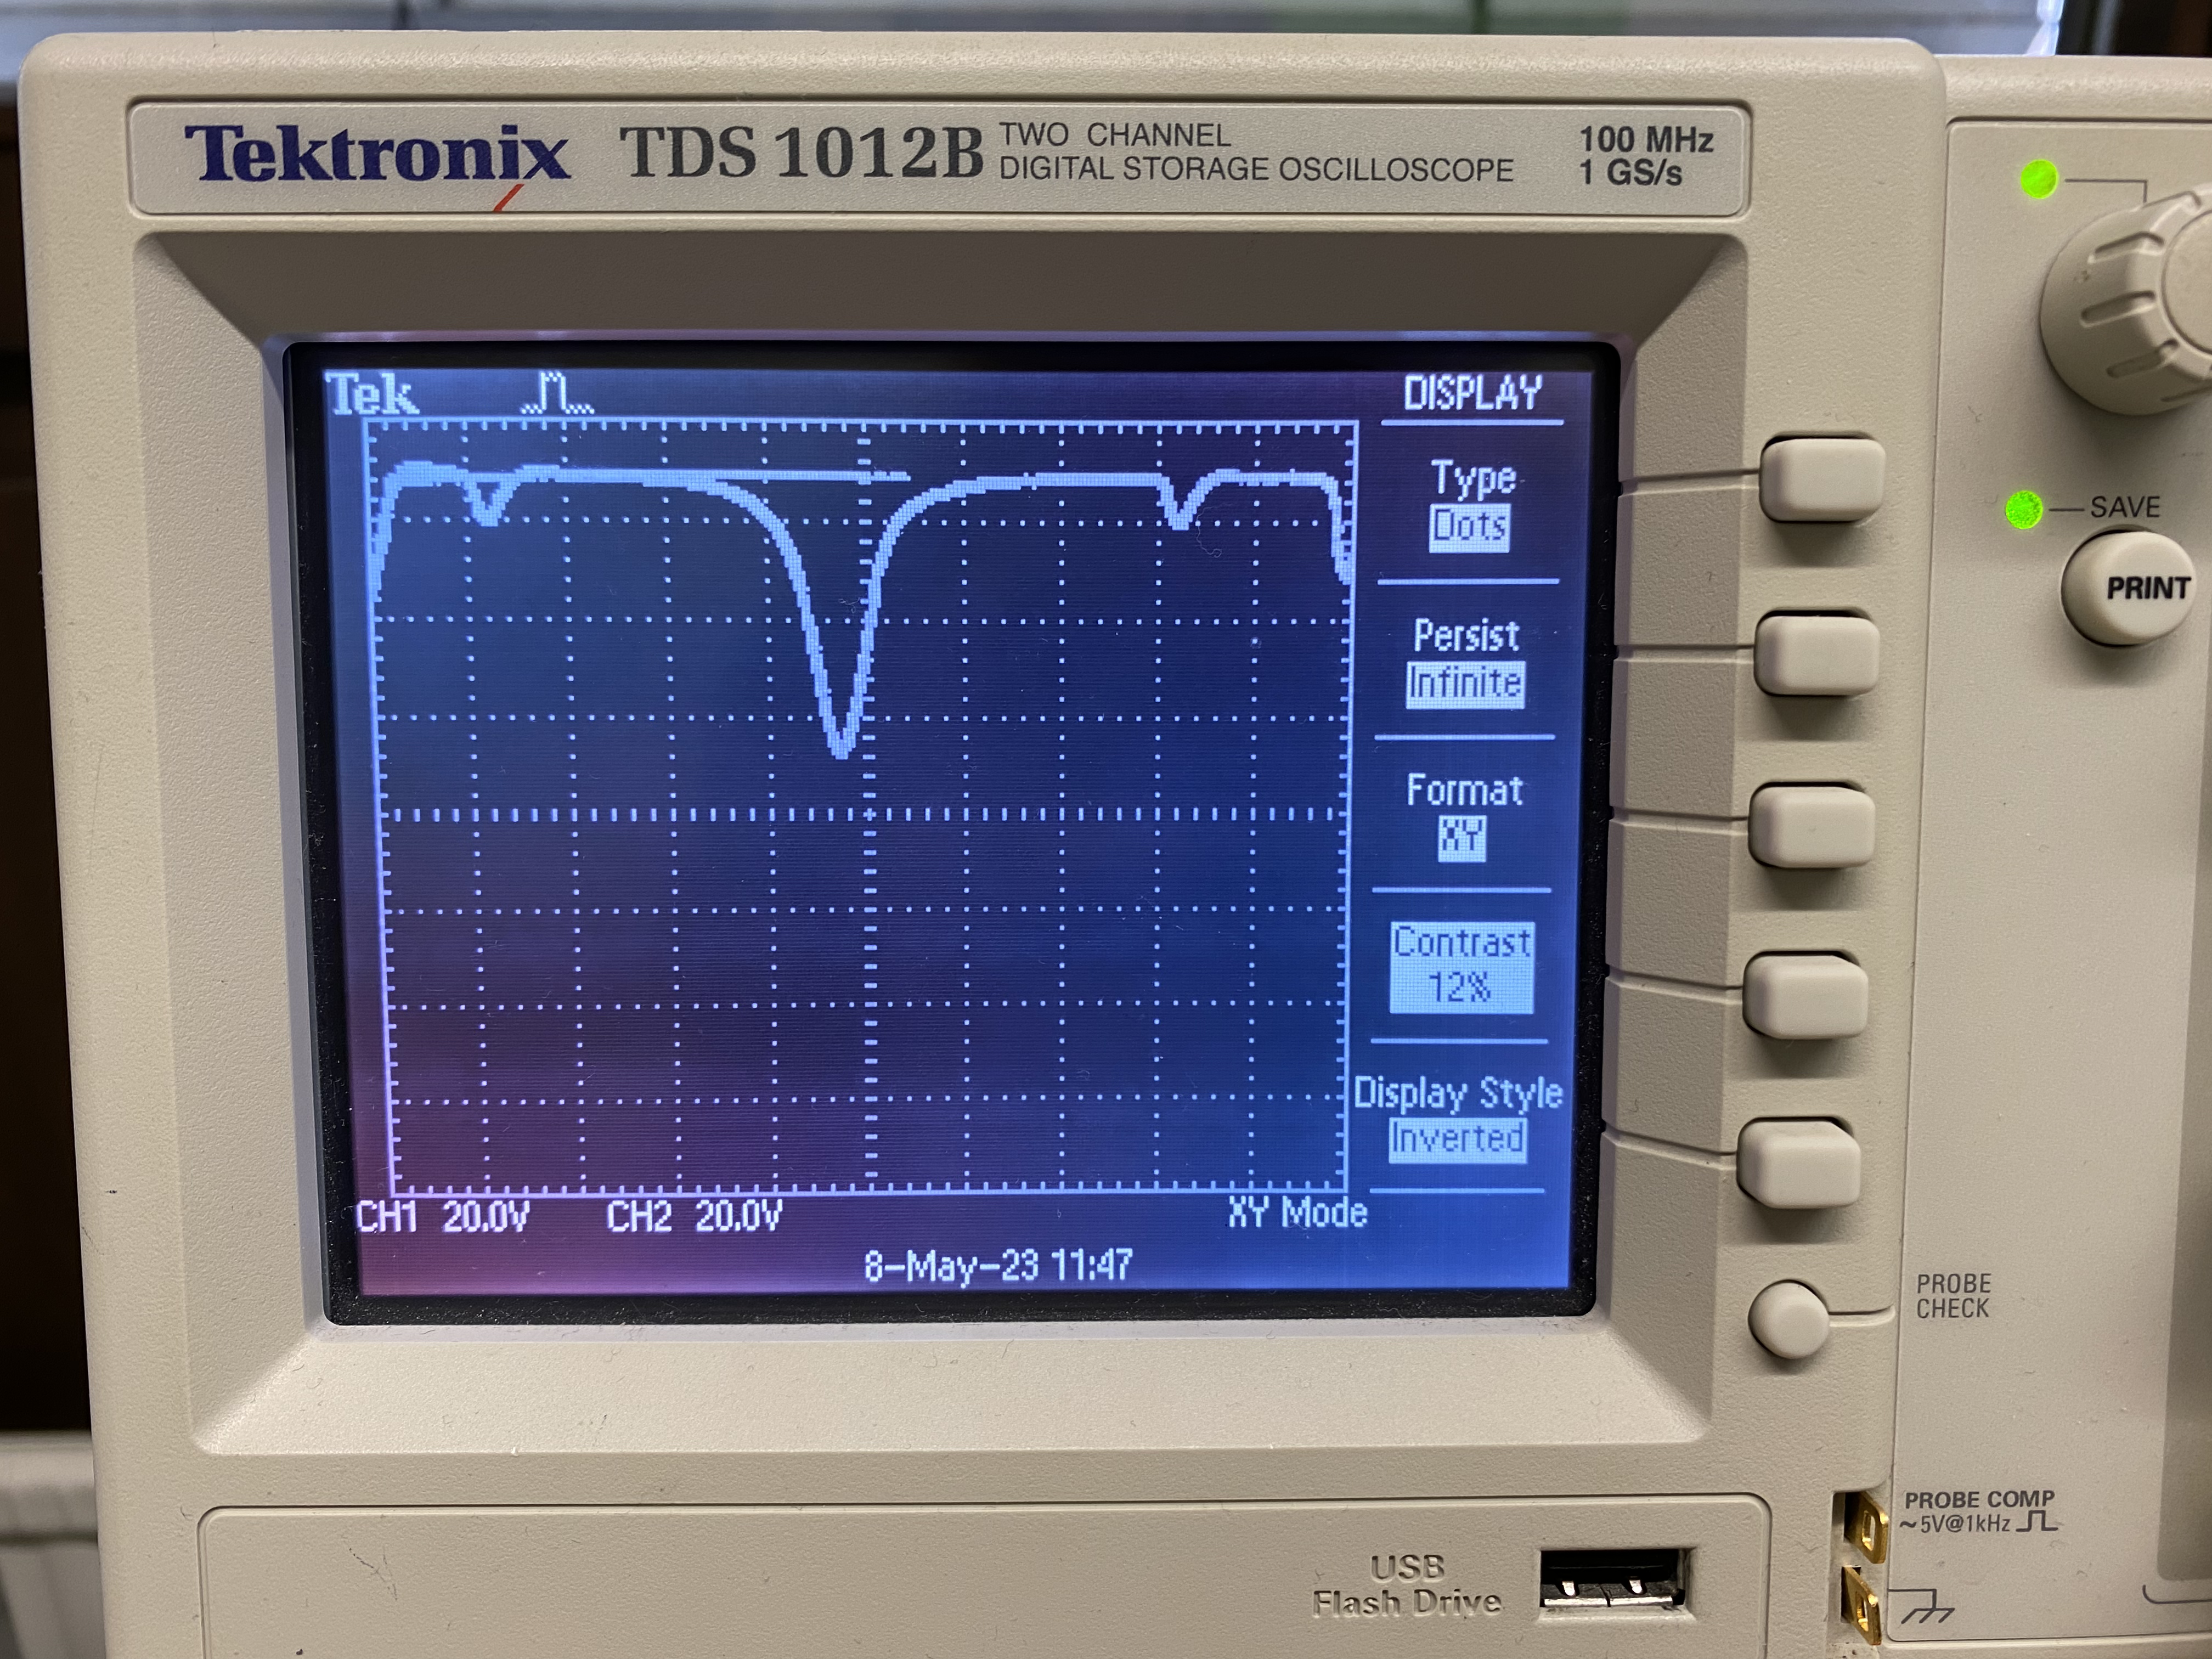
\includegraphics{data/Oszilloskop.png}
    \caption{Fotografie des Signalverlaufs bei $\SI{100}{\kilo\hertz}$.}
    \label{fig:Oszilloskop}
\end{figure}